\documentclass[pdf, fleqn, compress, handout]{beamer}
\usepackage{york_beamer_template}
\usepackage{tikz-cd}
\usepackage{frcursive}
\usepackage{mathrsfs}

\usetikzlibrary{shapes}

\newcommand{\arr}{\text{\textsl{\textcursive{r}}}}

\newcommand{\nord}[1]{\boldsymbol{:}\!#1\!\boldsymbol{:}}

\newcommand{\mathsterm}[1]{{\itshape\color{dark-teal!80}#1}}

\newcommand{\ourex}[1]{{\itshape\color{viridian!70!black}#1}}

\graphicspath{{/../fig/}}

\setlist[itemize,1]{itemsep=1em, leftmargin=0em}
\setitemize{label=\usebeamerfont*{itemize item}%
  \usebeamercolor[dark-teal!50!ebor]{itemize item}
  \usebeamertemplate{itemize item}}

\title[Graduate Research Symposium 2020]{The Casimir Effect in pAQFT: \\
\large Another `Argument' for $\boldsymbol{1 + 2 + 3 + ... = - 1/12}$}
\author[Sam Crawford]{Sam Crawford\\
Supervisors: Kasia Rejzner and Beno\^it Vicedo}
\date{\today}

\begin{document}

\begin{nonavigation}
%-------------------------------------------------------------------
%   Begin Frontmatter (Frames here have no head/foot and no logo)
%-------------------------------------------------------------------

\begin{frame}
    \titlepage
\end{frame}

%-------------------------------------------------------------------
%   End Frontmatter
%-------------------------------------------------------------------
\end{nonavigation}

\section{Intro: The Casimir Effect}

\begin{frame}{The Casimir Effect}
	\begin{columns}
		\column{0.7\textwidth}
			\begin{itemize}
				\item	\textbf{Experimentally:}
				\begin{itemize}
					\item	Metal plates, placed close together in a vacuum, attract
					\item	Explained by the presence of `fewer' quantum fluctuations
							of the vacuum within the cavity than without.
				\end{itemize}
				\item	\textbf{Theoretically:}
				\begin{itemize}
					\item	Discrepancy between the \mathsterm{normally ordered}
							energy-density of a spatially non-compact universe and
							a spatially compact one.
				\end{itemize}
			\end{itemize}
		\column{0.3\textwidth}
			\begin{figure}
				\centering
				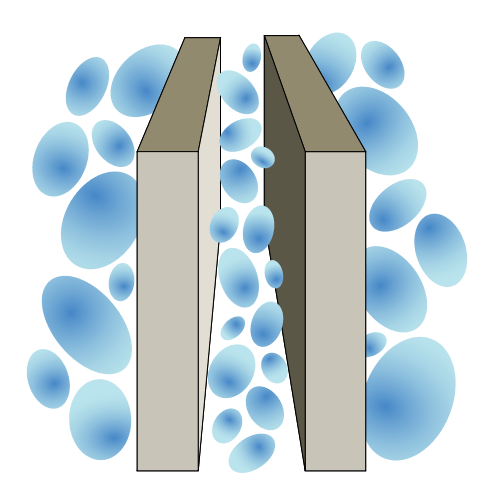
\includegraphics[width=\linewidth]{./fig/casimir.png}
			\end{figure}
	\end{columns}
\end{frame}

\section{Observables}

\begin{frame}{Classical Observables}
	\begin{itemize}
		\item	\mathsterm{Fields:}
					Smooth maps from spacetime $\mathcal{M}$ to $\mathbb{R}$
		\item	$\mathcal{C}^\infty(\mathcal{M})$ space of field configurations
		\item	\mathsterm{Classical observables:}
				Maps
				$\mathcal{F}: \mathcal{C}^\infty(\mathcal{M}) \to \mathbb{C}$
		\item	$\mathfrak{F}_\mathrm{loc}(\mathcal{M})$ space of `nice'
				classical observables.
	\end{itemize}
\end{frame}

\begin{frame}{Quantum Observables}
	\begin{itemize}
		\item	Actual quantum algebra, $\mathfrak{A}(\mathcal{M})$,
				defined abstractly
		\item	Given a \mathsterm{Hadamard distribution} $H$,
				get an associated isomorphism
				\begin{equation}
					\alpha_H:
					\mathfrak{A}(\mathcal{M})
						\to
					\left(
						\mathfrak{F}_{\mu c}(\mathcal{M}),
						\star_H
					\right)
						=:
					\mathfrak{A}^H(\mathcal{M})
				\end{equation}
		\item	For now, think of Hadamard distributions
				as \textbf{almost} smooth functions in
				$\mathcal{C}^\infty(\mathcal{M}^2)$
		\item	$\alpha_H$ defined formally,
				but for two Hadamard distributions $H, H'$,
				the map $\alpha_{H'} \circ \alpha_{H}^{-1} = \alpha_{H' - H}$
				is a well defined automorphism of
				$\mathfrak{F}_{\mu c}(\mathcal{M})$.
	\end{itemize}
\end{frame}

\begin{frame}{Comparing Classical to Quantum}
	\begin{itemize}
		\item	$\star$ product of quantum algebra non-commutative unlike
				pointwise product $\cdot$ of classical
		\item	$\rightsquigarrow$ ordering ambiguities when associating
				quantum counterpart to a classical observable
		\begin{itemize}
			\item	E.g. should $\mathcal{F} \cdot \mathcal{G}$ become
					$\mathcal{F} \star_H \mathcal{G}$, 
					$\mathcal{G} \star_H \mathcal{F}$, etc...
		\end{itemize}
		\item	A choice of map
				$
					\mathfrak{F}_\mathrm{loc}(\mathcal{M})
						\to
					\mathfrak{A}(\mathcal{M})
				$
				called an \mathsterm{ordering prescription}
		\item   Annoyingly denoted $\mathcal{F} \mapsto \nord{\mathcal{F}}$
	\end{itemize}
\end{frame}

\section{Comparison Across Spacetimes}

\begin{frame}{When Can We Compare Physics?}
	\begin{itemize}
		\item	Call a smooth map $\chi: \mathcal{M} \to \mathcal{N}$ an
				\mathsterm{admissible embedding} if it preserves
				geometry and causality
		\item	Prototyipical example is the inclusion
				$\iota: U \hookrightarrow \mathcal{M}$
				of a causally convex open subset
				$U \subset \mathcal{M}$
		\item	Think of $\mathcal{M}$ as a ``sub-spacetime'' of $\mathcal{N}$
	\end{itemize}
\end{frame}

\begin{frame}[fragile]{Comparing Classical Observables}
	\begin{itemize}
		\item	If $\phi \in \mathcal{C}^\infty(\mathcal{N})$, then
				$\chi^* \phi := \phi \circ \chi \in \mathcal{C}^\infty(\mathcal{M})$
		\item	Hence,
				$
					\chi_* \mathcal{F}[\phi]
						:=
					\mathcal{F}[\phi \circ \chi]	
				$
				is a classical observable in
				$\mathfrak{F}_\mathrm{loc}(\mathcal{N})$
		\item	Hence for every admissible embedding of spacetimes,
				we have an associated embedding of classical observables
		\begin{equation}
				\begin{tikzcd}
					\mathfrak{F}_\mathrm{loc}(\mathcal{M})
					\rar["\chi_*"] &
					\mathfrak{F}_\mathrm{loc}(\mathcal{N})
				\end{tikzcd}			
		\end{equation}
	\end{itemize}
\end{frame}

\begin{frame}[fragile]{Comparing Quantum Observables}
	\begin{itemize}
		\item	Difficult to define homomorphisms
				$\mathfrak{A}(\mathcal{M}) \to
				 \mathfrak{A}(\mathcal{N})$ directly
		\item	For
				$H  \in \mathrm{Had}(\mathcal{M})$,
				$H' \in \mathrm{Had}(\mathcal{N})$,
				we \textbf{can} write down a homomorphism
				$\mathfrak{A}^H(\mathcal{M}) \to \mathfrak{A}^{H'}(\mathcal{N})$
				\begin{equation}
					\mathcal{F}
						\mapsto
					\chi_* \left( \alpha_{\chi^* H' - H} \mathcal{F} \right)
				\end{equation}
				Which works because $\chi^* H' \in \mathrm{Had(\mathcal{M})}$.
		\item   Abstract homomorphism
				$
					\mathfrak{A}\chi:
					\mathfrak{A}(\mathcal{M})
						\to
					\mathfrak{A}(\mathcal{N})
				$
				then defined to make the following diagram commute
				\begin{equation}
					\begin{tikzcd}
						\mathfrak{A}(\mathcal{M})
							\ar[r, "\mathfrak{A}\chi"]
							\dar["\alpha_H"]	&
						\mathfrak{A}(\mathcal{N})
							\dar["\alpha_{H'}"]	\\
						\mathfrak{A}^H(\mathcal{M})
							\rar[
									swap,
									"\chi_* \circ \alpha_{\chi^* H' - H}",
									outer sep=5pt
								]	&
						\mathfrak{A}^{H'}(\mathcal{N})
					\end{tikzcd}
				\end{equation}
	\end{itemize}
\end{frame}

\begin{frame}[fragile]{Normal Ordering}
	\begin{itemize}
		\item	Define an ordering prescription
				$
					\nord{-}_\mathcal{M}:
					\mathfrak{F}_\mathrm{loc}(\mathcal{M})
						\to
					\mathfrak{A}(\mathcal{M})
				$
				for every spacetime $\mathcal{M}$
		\item   \mathsterm{Locally covariant Wick ordering}
				`compatible' with the maps defined earlier,
				i.e. the following diagram commutes
				\begin{equation}
					\begin{tikzcd}
						\mathfrak{F}_\mathrm{loc}(\mathcal{M})
							\rar["\chi_*"]
							\dar[swap, "\nord{-}_\mathcal{M}"]	&
						\mathfrak{F}_\mathrm{loc}(\mathcal{N})
							\dar["\nord{-}_\mathcal{N}"]	\\
						\mathfrak{A}(\mathcal{M})
							\rar[swap, "\mathfrak{A}\chi"]	&
						\mathfrak{A}(\mathcal{N})						
					\end{tikzcd}
				\end{equation}
		\item	Details of these maps actually irrelevant.
		\item   We only need to know (i) they exist,
				and (ii) they make the above diagram commute
	\end{itemize}
\end{frame}

\section{Doing the Calculation}

\begin{frame}{Stress-Energy on the Cylinder}
	\begin{itemize}
		\item	Spacetime: The Minkowski Cylinder
		\begin{itemize}
			\item	Minkowski space $\mathbb{M} \simeq \mathbb{R}^2$
			\item	Minkowski cylinder
					$\mathcal{M}_\mathrm{cyl} \simeq \mathbb{M} / \sim$,
					where $(t, x) \sim (t, x + 2\pi)$
			\item   Also introduce \mathsterm{null coordinates} $u = t + x$, $v = t - x$.
		\end{itemize}
		\item   For any point $\mathbf{x}_0 \in \mathbb{M}$,
				can define the \textbf{classical} observable
				\begin{equation}
					T_{\mathbf{x}_0}[\phi]
						:=
					\frac{1}{2}
					\left(
						\frac{\partial \phi}{\partial u}
						\Big|_{\mathbf{x} = \mathbf{x}_0}
					\right)^2,
				\end{equation}
				physically interpreted as (part of)
				the energy density for a massless scalar field.
	\end{itemize}
\end{frame}

\begin{frame}[fragile]{}
	\begin{columns}
		\begin{column}{0.5\textwidth}
			\begin{tikzpicture}[scale=1.5]
				% Axes
				\draw[->, thick] (0,   -2) -- (0,   2) node (yaxis) [left ] {$t$};
				\draw[->, thick] (-1.8, 0) -- (1.8, 0) node (xaxis) [below] {$x$};
				% Identification lines
				\draw[dashed] (1, -2) -- (1, 0) node (2pi) [below left] {$2\pi$}
								-- (1, 2);
				\draw[dashed] (-1, -2) -- (-1, 0) node (2pi) [below left] {$-2\pi$}
								-- (-1, 2);
				% Causal neighbourhood
				\node[
					diamond,
					fill=dark-teal!20,
					minimum size=40pt,
				] at (0.5,0.6) {$U$};
				% Basepoint and images
				\node[
					circle,
					fill=black,
					minimum size=3pt,
					inner sep=0pt,
					label=below :{$x_0$}
				] at (0.7, 0.5) {};
				\node[
					circle,
					fill=gray,
					minimum size=3pt,
					inner sep=0pt
				] at (1.7, 0.5) {};
				\node[
					circle,
					fill=gray,
					minimum size=3pt,
					inner sep=0pt
				] at (-0.3, 0.5) {};
				\node[
					circle,
					fill=gray,
					minimum size=3pt,
					inner sep=0pt
				] at (-1.3, 0.5) {};
			\end{tikzpicture}
		\end{column}
		\begin{column}{0.5\textwidth}
			\begin{tikzcd}
				\mathfrak{F}_\mathrm{loc}(U)
					\rar["\chi_*"]
					\dar[swap, "\nord{-}_U"]	&
				\mathfrak{F}_\mathrm{loc}(\mathcal{M}_\mathrm{cyl})
					\dar["\nord{-}_{\mathcal{M}_\mathrm{cyl}}"]	\\
				\mathfrak{A}(U)
					\rar[	swap,
							"\mathfrak{A}\chi"
					]
					\dar[
							swap,
							"\alpha_H"
					]
						&
				\mathfrak{A}(\mathcal{M}_\mathrm{cyl})
					\dar{
							\alpha_{H'}
					}
					\\
				\mathfrak{F}_{\mu c}(U)
					\rar[
							swap,
							outer sep=1ex,
							"\chi_* \circ \alpha_{\chi^* H' - H}"
					]	&
				\mathfrak{F}_{\mu c}(\mathcal{M}_\mathrm{cyl})
			\end{tikzcd}
		\end{column}
	\end{columns}
\end{frame}

\begin{frame}{Minkowski's Special}
	\begin{itemize}
		\item	There is a special Hadamard distribution
				$H_\mathbb{M} \in \mathrm{Had}(\mathbb{M})$,
				called the \mathsterm{Minkowski vacuum}.
		\item   In null coordinates, it can be written as
				\begin{equation*}
					H_\mathbb{M}(u, v; u', v')
						=
					\frac{1}{4 \pi}
					\int_{k = 0}^\infty
						\frac{1}{k}
						\left( 
							e^{-ik(u - u')} +
							e^{-ik(v - v')}
						\right)
					\, \mathrm{d}k
				\end{equation*}
		\item	Has the special property that
				$
					\alpha_{H_\mathbb{M}}\left(
						\nord{\mathcal{F}}_\mathbb{M}
					\right)
						=
					\mathcal{F}
				$,
				$
					\forall \mathcal{F}
						\in
					\mathfrak{F}_\mathrm{loc}(\mathbb{M})
				$.
		\item   So the ``left-hand column'' of the previous diagram
				becomes trivial.
	\end{itemize}
\end{frame}

\begin{frame}{Those $\boldsymbol{\alpha}$ Maps...}
	\begin{itemize}
		\item	In general, the map $\alpha_h$ is defined for any
				$h \in \mathcal{C}^\infty(\mathcal{M}^2)$ by
				\begin{equation*}
					\mathcal{\alpha}_h(\mathcal{F})
						=
					\sum_{n = 0}^\infty
						\frac{\hbar^n}{2^n n!}
						\int_{\mathcal{M}^{2n}}
						\prod_{i = 1}^n h(\mathbf{x}_i; \mathbf{y}_i)
						\frac{
								\delta^{2n} \mathcal{F}
							}{
								\delta \phi(\mathbf{x}_1)
									\cdots
								\delta \phi(\mathbf{y}_n)						
							}
						\, \mathrm{dV}^{2n}
				\end{equation*}
		\item	For $T_{\mathbf{x}_0}$ we have
				\begin{equation}
					\frac{
							\delta^2 T_{\mathbf{x}_0}
						}{
							\delta \phi(\mathbf{x})
							\delta \phi(\mathbf{y})
						}
						=
					\partial_u \delta(\mathbf{x}_0 - \mathbf{x})
					\partial_{u'} \delta(\mathbf{x} - \mathbf{y})
				\end{equation}
		\item   Which simplifies the above map to
				\begin{equation}
					\alpha_h(T_{\mathbf{x}_0})
						=
					T_{\mathbf{x}_0}
						+
					\frac{\hbar}{2}
					\partial_u \partial_{u'}
					h(\mathbf{x}_0; \mathbf{x}_0)
				\end{equation}
	\end{itemize}
\end{frame}

% \section{Old Shite}

% \begin{frame}{Some Terminology}
% 	\begin{itemize}
% 		\item	\mathsterm{Spacetime}: A smooth pseudo-Riemannian manifold
% 				$\mathcal{M}$.
% 				It is \mathsterm{globally hyperbolic} if it can be written
% 				\begin{equation}
% 					\mathcal{M}
% 						\simeq
% 					\underbrace{\mathbb{R}}_{\text{time}}
% 						\times
% 					\underbrace{\Sigma}_{\text{space}}.
% 				\end{equation}
% 		\vspace{-0.5em}
% 		\pause

% 				\ourex{
% 				E.g. the 2D globally hyperbolic cylinder
% 				$\mathcal{M}_\mathrm{cyl} = \mathbb{R} \times S^1$.
% 				}
% 		\pause
% 		\item	\mathsterm{Field}: Generally a smooth section of some fibre bundle.
		
% 		\pause
% 				\ourex{For us simply a smooth, real-valued function
% 				$\phi \in \mathcal{C}^\infty(\mathcal{M})$.}
% 		\pause
% 		\item	\mathsterm{(Classical) Observable:} A functional
% 				$\mathcal{F}: \mathcal{C}^\infty(\mathcal{M}) \to \mathbb{C}$. 

% 				\ourex{E.g. The stress-energy at
% 						$(t_0, x_0) = \mathbf{x}_0 \in \mathcal{M}_\mathrm{cyl}$}
% 				\ourex{
% 					\begin{equation}
% 						T_{\mathbf{x}_0}[\phi]
% 							:=
% 						\frac{1}{2}
% 						{\underbrace{
% 						\left(
% 							\frac{\partial \phi}{\partial t} +
% 							\frac{\partial \phi}{\partial x}
% 						\right)
% 						}_{\partial \phi}}^2
% 						(t_0, x_0)					
% 					\end{equation}
% 				}
% 	\end{itemize}
% \end{frame}

% \begin{frame}{A \textit{Little} Functional Analysis}
% 	\begin{itemize}
% 		\item	Just as we ask $\phi$ to be smooth,
% 				we can impose smoothness on the functionals.
% 		\item	The derivative of
% 				$\mathcal{F}$ at $\phi \in \mathcal{C}^\infty(\mathcal{M})$
% 				in the direction $h    \in \mathcal{C}^\infty(\mathcal{M})$ is
% 				\begin{equation}
% 					\left\langle 
% 						\mathcal{F}^{(1)}[\phi]
% 							,
% 						h
% 					\right\rangle
% 						:=
% 						\lim_{\epsilon \to 0}
% 							\frac{
% 								\mathcal{F}[\phi + \epsilon h] - \mathcal{F}[\phi]
% 							}{
% 								\epsilon
% 							},
% 				\end{equation}
% 				wherever this limit exists.
% 		\item 	If it exists $\forall \phi, h \in \mathcal{C}^\infty(\mathcal{M})$,
% 				then $\mathcal{F}^{(1)}$ is a map from
% 				field configurations to \mathsterm{distributions}
% 				(a.k.a. `generalised functions')
		
% 				\ourex{
% 					E.g. for $T_{\mathbf{x}_0}$ as before we have
% 					\begin{align}
% 						\left\langle
% 							T_{\mathbf{x}_0}^{(1)}[\phi],
% 							h
% 						\right\rangle
% 							&=
% 						\partial \phi(\mathbf{x}_0)
% 						\partial   h (\mathbf{x}_0)
% 					\end{align}
% 					}
% 	\end{itemize}
% \end{frame}

% \begin{frame}{A Little More Functional Analysis}
% 	\begin{itemize}
% 		\item	Notational aside: For a distribution
% 				$S \in {\mathcal{C}^\infty}'(\mathcal{M}^n)$
% 				\begin{equation*}
% 					\left\langle
% 						S,
% 						h_1 \otimes \cdots \otimes h_n
% 					\right\rangle
% 						=
% 					\int_{\mathcal{M}^n}
% 						S(\mathbf{x}_1, \ldots, \mathbf{x}_n)
% 						h_1(\mathbf{x}_1) \cdots h_n(\mathbf{x}_n)
% 					\, \mathrm{dV}^n					
% 				\end{equation*}
% 		\vspace{-1em}
% 		\pause
% 		\item	$\mathcal{F}$ is \mathsterm{smooth} if $\mathcal{F}^{(n)}$
% 				exists $\forall n \in \mathbb{N}$.
% 		\pause
% 		\item	$\mathfrak{F}_\mathrm{reg}(\mathcal{M})$ the set of
% 				\mathsterm{regular} functionals, defined such that
% 				$\mathcal{F}^{(n)}[\phi]$ a \textit{bona fide} smooth function for all
% 				$n   \in \mathbb{N},
% 				\phi \in \mathcal{C}^\infty(\mathcal{M})$.
% 		\vspace{1em}

% 		\pause
% 				\ourex{E.g. for $T_{\mathbf{x}_0}$ as before
% 				\begin{itemize}
% 					\item	$
% 								T_{\mathbf{x}_0}^{(1)}[\phi](\mathbf{x})
% 									=
% 								-\partial(\delta(\mathbf{x} - \mathbf{x}_0)
% 								 \partial \phi  (\mathbf{x}))
% 							$
% 					\item	$
% 								T_{\mathbf{x}_0}^{(2)}[\phi](\mathbf{x}; \mathbf{y})
% 									=
% 								-\partial(\delta(\mathbf{x} - \mathbf{x}_0)
% 								 \partial (\delta(\mathbf{x} - \mathbf{y})))
% 							$
% 					\item	$
% 								T_{\mathbf{x}_0}^{(n)}[\phi] = 0
% 							$,
% 							for $n > 2$.
% 				\end{itemize}
% 				So $T_{\mathbf{x}_0}$ is smooth, but not regular.
% 				}
% 	\end{itemize}
% \end{frame}

% \begin{frame}{Classical Dynamics}
% 	\begin{itemize}
% 		\item	Choice of field theory encapsulated in \mathsterm{Poisson bracket}
% 				\begin{align}
% 					\{\cdot, \cdot\}:
% 					\mathfrak{F}_\mathrm{reg}(\mathcal{M})
% 						\otimes
% 					\mathfrak{F}_\mathrm{reg}(\mathcal{M})
% 						&\to
% 					\mathfrak{F}_\mathrm{reg}(\mathcal{M}), \nonumber \\
% 					(\mathcal{F}, \mathcal{G})
% 						&\mapsto
% 					\left\langle 
% 						E,
% 						\mathcal{F}^{(1)}
% 							\otimes
% 						\mathcal{G}^{(1)}
% 					\right\rangle.
% 				\end{align}
% 		\item	$E(\mathbf{x}; \mathbf{y}) \in {\mathcal{C}^\infty}'(\mathcal{M}^2)$
% 				a bi-distribution called the \mathsterm{causal propagator}.	
	
% 		\vspace{1em}
% 				\ourex{Causal propagator for the massless scalar field on $\mathcal{M}_\mathrm{cyl}$
% 				\begin{equation}
% 					E(u, v; u', v')
% 						=
% 					% Without summation:
% 					% -\frac{1}{2}
% 					% \left(
% 					% 	\left\lfloor
% 					% 		\frac{u - u'}{2\pi}
% 					% 	\right\rfloor +
% 					% 	\left\lfloor
% 					% 		\frac{v - v'}{2\pi}
% 					% 	\right\rfloor +
% 					% 	1
% 					% \right).
% 					%---------------------------------------
% 					% With summation:
% 					\frac{i}{4 \pi}
% 					\sum_{n \in \mathbb{Z}^*}
% 						\frac{1}{k}
% 						\left(
% 							e^{-ik(u - u')} +
% 							e^{-ik(v - v')}
% 						\right)
% 				\end{equation}
% 				}
% 	\end{itemize}
% \end{frame}

% % ----------------------------------------
% %		Too much detail for time
% % ----------------------------------------
% % \begin{frame}{Classical Dynamics}
% % 	\begin{itemize}
% % 		\item	Laws of physics $\rightsquigarrow$
% % 				\mathsterm{equations of motion (EoM)} $\rightsquigarrow$
% % 				distinguished bi-solution, called the \mathsterm{causal propagator},
% % 				denoted $E$.
		
% % 		\vspace{1em}
% % 				\ourex{For the massless scalar field on $\mathcal{M}_\mathrm{cyl}$, the equation of motion is
% % 				\begin{equation}
% % 					\partial_t^2\phi - \partial_x^2 \phi
% % 						=
% % 					4\partial_u \partial_v \phi
% % 						=
% % 					0,
% % 					\qquad \qquad (u, v = t \pm x)
% % 				\end{equation}
% % 				for which we have the causal propagator
% % 				\begin{equation}
% % 					E(u, v; u', v')
% % 						=
% % 					% Without summation:
% % 					% -\frac{1}{2}
% % 					% \left(
% % 					% 	\left\lfloor
% % 					% 		\frac{u - u'}{2\pi}
% % 					% 	\right\rfloor +
% % 					% 	\left\lfloor
% % 					% 		\frac{v - v'}{2\pi}
% % 					% 	\right\rfloor +
% % 					% 	1
% % 					% \right).
% % 					%---------------------------------------
% % 					% With summation:
% % 					\frac{i}{4 \pi}
% % 					\sum_{n \in \mathbb{Z}^*}
% % 						\frac{1}{k}
% % 						\left(
% % 							e^{-ik(u - u')} +
% % 							e^{-ik(v - v')}
% % 						\right)
% % 				\end{equation}
% % 				}
% % 		\vspace{-1em}
% % 		\item	Causal propagator $\rightsquigarrow$ \mathsterm{Poisson bracket}
% % 				\begin{align}
% % 					\{\cdot, \cdot\}:
% % 					\mathfrak{F}_\mathrm{reg}(\mathcal{M})
% % 						\otimes
% % 					\mathfrak{F}_\mathrm{reg}(\mathcal{M})
% % 						&\to
% % 					\mathfrak{F}_\mathrm{reg}(\mathcal{M}), \nonumber \\
% % 					(\mathcal{F}, \mathcal{G})
% % 						&\mapsto
% % 					\left\langle 
% % 						E,
% % 						\mathcal{F}^{(1)}
% % 							\otimes
% % 						\mathcal{G}^{(1)}
% % 					\right\rangle.
% % 				\end{align}
% % 	\end{itemize}
% % \end{frame}

% \begin{frame}{The Poisson Bracket}
% 	\vspace{-2em}
% 	\begin{equation}
% 		\{\mathcal{F}, \mathcal{G}\}[\phi]
% 			= 
% 		\left\langle 
% 			E,
% 			\mathcal{F}^{(1)}[\phi]
% 				\otimes
% 			\mathcal{G}^{(1)}[\phi]
% 		\right\rangle
% 	\end{equation}
% 	\begin{itemize}
% 		\item	Can be extended to the space of \mathsterm{microcausal} functionals
% 				$\mathfrak{F}_{\mu \mathrm{c}}(\mathcal{M}) \supset 
% 				\mathfrak{F}_\mathrm{reg}(\mathcal{M})$
% 		\pause
% 		\item	Importantly, $\mathfrak{F}_{\mu \mathrm{c}}(\mathcal{M})$ contains
% 				\mathsterm{local} observables such as \ourex{$T_{\mathbf{x}_0}$},
% 		\pause
% 		\item	and also $\mathfrak{F}_\mathrm{reg}(\mathcal{M})$ as a \textbf{dense} subspace
% 		\pause
% 		\item	Poisson bracket is the key ingredient from classical theory for quantisation.
% 	\end{itemize}
% \end{frame}

% \begin{frame}{Quantisation}
% 	\begin{itemize}
% 		\item	In pAQFT, quantisation is the \textit{deformation} of
% 				the pointwise product $\cdot$ on $\mathfrak{F}_*(\mathcal{M})$ into a new,
% 				associative product $\star$ such that
% 				\begin{itemize}
% 					\item[(i)] $\mathcal{F} \star \mathcal{G} = \mathcal{F} \cdot \mathcal{G} + \hbar \cdots$
% 					\item[(ii)] $
% 								\mathcal{F} \star \mathcal{G} -
% 								\mathcal{G} \star \mathcal{F} =
% 								i\hbar \{\mathcal{F}, \mathcal{G}\} +
% 								\hbar^2 \cdots
% 								$
% 				\end{itemize}
% 		\pause
% 		\item	$\hbar$ a formal parameter (i.e. don't think too much about convergence)
% 		\begin{itemize}
% 			\item	So new algebra is in fact
% 					$\left(\mathfrak{F}_*(\mathcal{M})[[\hbar]], \star \right)$
% 		\end{itemize}
% 	\end{itemize}
% \end{frame}

% \begin{frame}{Ordering Ambiguity}
% 	\begin{itemize}
% 		\item	\textbf{What should the quantum analogue of}
% 				$\mathcal{F} \cdot \mathcal{G}$ \textbf{be?}
% 		\pause
% 		\item	Options include
% 				$\mathcal{F} \star \mathcal{G}$,
% 				$\mathcal{G} \star \mathcal{F}$,
% 				$\frac{1}{2} \left( 
% 				\mathcal{F} \star \mathcal{G} + 
% 				\mathcal{G} \star \mathcal{F} \right)
% 				$, etc...
% 		\pause
% 		\item	Map from classical to quantum observables called an
% 				\mathsterm{ordering precription}.
% 		\pause
% 		\item   Therefore two separate tasks:
% 		\begin{itemize}
% 			\item[(i)] Find quantum algebra
% 			\item[(ii)] Find map from classical to quantum algebra
% 		\end{itemize}
% 	\end{itemize}
% \end{frame}

% \begin{frame}{The Star Product}
% 	\begin{itemize}
% 		\item	The star product used in pAQFT is (for a non-interacting theory)
% 				\begin{equation}
% 					\mathcal{F} \star_W
% 					\mathcal{G}
% 						:=
% 					\mathcal{F} \cdot
% 					\mathcal{G}
% 						+
% 					\sum_{n = 1}^\infty
% 					\frac{\hbar^n}{n!}
% 					\left\langle 
% 						\!\left( \tfrac{i}{2} E + H \right)^{\otimes n},
% 						\mathcal{F}^{(n)} \otimes
% 						\mathcal{G}^{(n)}
% 					\right\rangle
% 				\end{equation}
% 				\begin{itemize}
% 					\item	$H$ is another distributional solution to the EoM.
% 					\item	Chosen so $\star$ product well-defined on
% 							$\mathfrak{F}_{\mu \mathrm{c}}(\mathcal{M})$.
% 				\end{itemize}
% 		\item	The sum $W = \tfrac{i}{2} E + H$ called a \mathsterm{Hadamard distribution}.
% 				Physically interpreted as `vacuum-like' solution to EoM.
% 	\end{itemize}
% \end{frame}

% \begin{frame}{Hadamard Distributions}
% 	\begin{itemize}
% 		\item	{\color{ebor}\bfseries Good News:}
% 				Hadamard distributions always exist on globally-hyperbolic spacetimes
% 		\pause

% 		\vspace{1em}
% 		\ourex{
% 				On the cylinder there is the \textit{ultrastatic vacuum state}
% 				\begin{align}
% 					W_\mathrm{cyl}(u, v; u', v')
% 						=
% 					\frac{1}{4 \pi}
% 					\sum_{k = 1}^\infty
% 						\frac{1}{k}
% 						\left( 
% 							e^{-ik(u - u')} +
% 							e^{-ik(v - v')}
% 						\right)
% 				% Not enough space, would be nice to show though
% 				% &		=
% 				% 	\frac{i}{8 \pi}
% 				% 	\left(
% 				% 		\sum_{k \in \mathbb{Z}^*}
% 				% 			\frac{1}{k}
% 				% 			\left( 
% 				% 				e^{ik(u - u')} +
% 				% 				e^{ik(v - v')}
% 				% 			\right) +
% 				% 		\sum_{k \in \mathbb{Z}^*}
% 				% 			\frac{1}{|k|}
% 				% 			\left( 
% 				% 				e^{ik(u - u')} +
% 				% 				e^{ik(v - v')}
% 				% 			\right)
% 				%	\right)
% 				\end{align}
% 				}
% 		\vspace{-1.5em}
% 		\pause
% 		\item	{\color{ebor}\bfseries Bad  News:}
% 				Infinitely many exist for every spacetime.
% 				In general with none being distinguished above the others.
% 		\pause
% 		\item	{\color{ebor}\bfseries Good News:}
% 				Different choices of $W$ yield isomorphic products,
% 				with the isomorphism given by
% 				\begin{equation}
% 					\alpha_{W' - W}(\mathcal{F})
% 						:=
% 					\mathcal{F}
% 						+
% 					\sum_{n = 1}^\infty
% 					\frac{\hbar^{n}}{2^{n} n!}
% 					\left\langle 
% 						(W' - W)^{\otimes n},
% 						\mathcal{F}^{(2n)}
% 					\right\rangle
% 				\end{equation}
% 	\end{itemize}
% \end{frame}

% \begin{frame}{Normal Ordering}
% 	\begin{itemize}
% 		\item	{\color{ebor}\bfseries Compromise:}
% 				Quantum algebra
% 				$
% 				\mathfrak{A}_W
% 					=
% 				\left(
% 					\mathfrak{F}_{\mu \mathrm{c}}(\mathcal{M})[[\hbar]],
% 					\star_W
% 				\right)
% 				$
% 				for some arbitrary choice of $W$,
% 				but use an ordering prescription relative to that choice.
% 		\pause
% 		\item	I.e. for every $W$, define $\nord{-}_W$ such that,
% 				for a classical observable $\mathcal{F}$
% 				\begin{equation}
% 					\alpha_{W' - W} (\nord{\mathcal{F}}_W)
% 						=
% 					\, \nord{\mathcal{F}}_{W'}.
% 				\end{equation}
% 		\pause \vspace{-2em}
% 		\item	For \mathsterm{local} observables,
% 				including \ourex{$T_{\mathbf{x}_0}$},
% 				can use the \mathsterm{Hadamard parametrix}.
% 	\end{itemize}
% \end{frame}

% \begin{frame}{Hadamard Parametrix}
% 	\begin{itemize}
% 		\item	A way of splitting the $W(\mathbf{x}; \mathbf{y})$ distributions as
% 				$
% 					W(\mathbf{x}; \mathbf{y})
% 						=
% 					w(\mathbf{x}; \mathbf{y}) + 
% 					W^\mathrm{sing}(\mathbf{x}; \mathbf{y})
% 				$
% 		\begin{itemize}
% 			\item	$w(\mathbf{x}; \mathbf{y})$ can be made $\mathcal{C}^N$ for arbitrarily large $N$.
% 		\end{itemize}
% 		\pause
% 		\item	For all Hadamard distributions,
% 				$w(\mathbf{x}; \mathbf{y})$
% 				only guaranteed to exist on some neighbourhood of
% 				$
% 					\{(\mathbf{x}, \mathbf{x}) \in \mathcal{M}^2
% 						|
% 					\mathbf{x} \in \mathcal{M}\}
% 				$,
% 		\begin{itemize}
% 			\item	But when defined, we have $W' - W = w' - w$,
% 			\item	I.e. $W^\mathrm{sing}$ is \textbf{the same} for all $W$.
% 		\end{itemize}				
% 		\pause
% 		\item	Ordering map then $\nord{\mathcal{F}}_W = \alpha_{w}(\mathcal{F})$.
% 		\pause

% 		\vspace{1em}
% 		\ourex{
% 				Parametrix for cylinder:
% 				\begin{equation*}
% 					W^\mathrm{sing}_\mathrm{cyl}(u, v; u', v')
% 						=
% 					\frac{1}{4 \pi}
% 					\int_{k = 0}^\infty
% 						\frac{1}{k}
% 						\left( 
% 							e^{-ik(u - u')} +
% 							e^{-ik(v - v')}
% 						\right)
% 					\, \mathrm{d}k
% 				\end{equation*}
% 		}
% 	\end{itemize}
% \end{frame}

% \begin{frame}{Ordering $T_{\mathbf{x}_0}$}
% 	\begin{itemize}
% 		\item 	Recall
% 				$
% 					\left\langle
% 						T_{\mathbf{x}_0}^{(2)},
% 						h_1 \otimes h_2
% 					\right\rangle
% 						=
% 					\partial h_1(\mathbf{x}_0)
% 					\partial h_2(\mathbf{x}_0)
% 				$
% 		\item   Hence, for any smooth function
% 				$h \in \mathcal{C}^{\infty}(\mathcal{M}_\mathrm{cyl}^2)$,
% 				\begin{align}
% 					\alpha_h \left( T_{\mathbf{x}_0} \right)
% 					&	=
% 					T_{\mathbf{x}_0}
% 						+
% 					\frac{\hbar}{2}
% 					\left\langle 
% 						h,
% 						T_{\mathbf{x}_0}^{(2)}
% 					\right\rangle
% 					\nonumber \\
% 					&	=
% 					T_{\mathbf{x}_0}
% 						+
% 					\frac{\hbar}{2}
% 					\lim_{\mathbf{y} \to \mathbf{x}}
% 						\left( \partial \otimes \partial \right) h(\mathbf{x}; \mathbf{y}).
% 				\end{align}
% 		\item   Hence, the `quantum correction' we must compute is
% 				\begin{equation}
% 					\frac{\hbar}{2}
% 					\lim_{u' \to u}
% 					\partial_u \partial_{u'}
% 					\left(
% 						W_\mathrm{cyl}(u, v; u', v) -
% 						W_\mathrm{cyl}^\mathrm{sing}(u, v; u', v)
% 					\right)
% 				\end{equation}
% 	\end{itemize}
% \end{frame}

\begin{frame}{Calculating the correction}
	\begin{itemize}
		\item	The two Hadamard distributions
				\begin{align*}
					\chi^*H_\mathrm{cyl}(u, v; u', v')
					&	=
					\frac{1}{4 \pi} \sum_{k = 1}^\infty
						\frac{1}{k} \left( 
							e^{-ik(u - u')} +
							e^{-ik(v - v')}
						 \right)
					\\
					H_\mathbb{M}(u, v; u', v')
					&	=
					\frac{1}{4 \pi} \int_{k = 0}^\infty
						\frac{1}{k} \left( 
							e^{-ik(u - u')} +
							e^{-ik(v - v')}
						 \right)
						\mathrm{d}k
				\end{align*}
		\item	By defining $z_\epsilon = \epsilon + i(u - u')$,
				can approximate by smooth functions:
				\begin{subequations}
					\begin{align}
						\label{eq:w_cyl_approx}
						\partial_u \partial_{u'}
						H_\mathrm{cyl}(u; u')
						&	=
						\frac{1}{4\pi}
						\lim_{\epsilon \to 0^+} \frac{e^{z_\epsilon}}{(1 - e^{z_\epsilon})^2}
							\\
						\partial_u \partial_{u'}
						H_\mathbb{M}(u; u')
						&	=
						\frac{1}{4\pi}
						\lim_{\epsilon \to 0^+}
							- \frac{1}{z_\epsilon^2}.
					\end{align}					
				\end{subequations}
	\end{itemize}
\end{frame}

\begin{frame}{Calculating the correction}
	\begin{itemize}
		\item	The RHS of \eqref{eq:w_cyl_approx} can be written as a Laurent series
				\begin{equation}					
					\frac{e^{z_\epsilon}}{(1 - e^{z_\epsilon})^2}
						=
					- \frac{1}{z_\epsilon^2}
					+ \sum_{n = 0}^\infty
							\frac{\zeta(-n - 1)}{n!} z_\epsilon^n
				\end{equation}
		\item	Hence the quantum correction we want is
				\begin{align*}
					\frac{\hbar}{2}
					\lim_{u' \to u}
					\partial_u \partial_{u'}
					\left(
						H_\mathrm{cyl} -
						H_\mathbb{M}
					\right)
					&	=
					\frac{\hbar}{8 \pi}
					\lim_{z_\epsilon \to 0}
						\sum_{n = 0}^\infty
							\frac{\zeta(-n - 1)}{n!} z_\epsilon^n 
						\\
					&	=
					\frac{\hbar}{8 \pi} \frac{-1}{12}
				\end{align*}
	\end{itemize}
\end{frame}

\begin{frame}{$\boldsymbol{1 + 2 + \cdots \overset{?}{=} -1/12}$}
	\begin{itemize}
		\item	Taking the $u' \to u$ limit na\"ively would instead give
				\begin{equation*}
					\frac{\hbar}{2}
					\lim_{u' \to u}
					\partial_u \partial_{u'}
					\left(
						W_\mathrm{cyl} -
						W_\mathbb{M}
					\right)
						\text{``} \! = \! \text{''}
					\frac{\hbar}{8\pi}
						\left( 
							\sum_{k = 1}^\infty k
								-
							\int_{k = 0}^\infty k \, \mathrm{d}k
						 \right).
				\end{equation*}
		\pause
		\item	So perhaps $\sum_\mathbb{N} k$ is not $-1 / 12$, but instead
				$\sum_\mathbb{N} k = -1 / 12 + \int_{\mathbb{R}_+} k \, \mathrm{d}k$...
	\end{itemize}
\end{frame}

\begin{nonavigation}
\appendix

\begin{frame}
	Thanks for listening!
\end{frame}

\end{nonavigation}

\end{document}